\section{随机过程}

\begin{kbox}{1. 随机过程定义与统计特性}
    \textbf{定义}:
    随时间作随机变化的一系列随机变量的集合。
        \begin{itemize}[leftmargin=3em]
            \item[(1)] 结构上是:所有样本函数 $\xi_i(t)$ 的集合;
            \item[(2)] 也是随机变量 $\xi(t)$ 的集合。
        \end{itemize}

    \tcbline

    \textbf{统计特性与物理意义}:
    \begin{itemize}
        \item \textbf{一维分布函数}:
        \[ F_1(x_1, t_1) = P\{\xi(t_1) \leq x_1\} \]
        \item \textbf{一维概率密度函数 (PDF)}:
        \[ f_1(x_1, t_1) = \frac{\partial F_1(x_1, t_1)}{\partial x_1} \]
        \item \textbf{均值 (数学期望)} —— \textcolor{mainblue}{直流分量}:
        \[ \mu(t) = E[\xi(t)] = \int_{-\infty}^{\infty} x f_1(x, t) dx \]
        \item \textbf{方差} —— \textcolor{mainblue}{交流功率}:
        \[ \sigma^2(t) = D[\xi(t)] = E\left[(\xi(t) - \mu(t))^2\right] \]
        \item \textbf{平均功率 (二阶原点矩)}:
        由 $DX = E(X^2) - (EX)^2$ 可知功率关系:
        \[ \underbrace{E[\xi^2(t)]}_{\text{平均功率}} = \underbrace{\sigma^2(t)}_{\text{交流功率}} + \underbrace{\mu^2(t)}_{\text{直流功率}} \]
        (当 $\mu(t)=0$ 时,平均功率等于交流功率)
        
        \item \textbf{自相关函数}:
        描述同一过程在任意两个时刻随机变量间的关联程度。
        \begin{align*}
            R(t_1, t_2) &= E[\xi(t_1)\xi(t_2)] \\
            &= \iint_{-\infty}^{\infty} x_1 x_2 f_2(x_1, x_2; t_1, t_2) dx_1 dx_2
        \end{align*}
        (其中 $f_2$ 为二维概率密度函数)
        
        \item \textbf{互相关函数}:
        \[ R_{\xi\eta}(t_1, t_2) = E[\xi(t_1)\eta(t_2)] \]
    \end{itemize}
\end{kbox}

% --- 核心概念辨析 ---
\begin{kbox}{核心概念辨析:样本函数 vs 随机变量}
    \textbf{误区}:随机过程的“样本”不是随机变量,二者观察维度不同。
    
    对于随机过程 $\xi(t, \omega)$:
    \begin{itemize}
        \item \textbf{样本函数 (Sample Function)}:\textcolor{alertred}{固定 $\omega$,变化 $t$}。
        \\ 指随机过程的\textbf{一次具体实现}(如做了一次实验记录下的波形)。既然实验已发生,它就是一条\textbf{确定的时间函数} $x(t)$,不再具有随机性。
        \item \textbf{随机变量 (Random Variable)}:\textcolor{alertred}{固定 $t$,变化 $\omega$}。
        \\ 指随机过程在\textbf{某一特定时刻}的状态。它包含该时刻所有可能的取值及其概率分布,是\textbf{随机的}。
        \item \textbf{总结}:样本函数是“时间的函数”,随机变量是“概率的函数”。二者同时固定时,唯一确定一个数值。
    \end{itemize}
    
    \tcbline
    
    \textbf{直观总结}:
    \begin{itemize}
        \item “样本”是\textbf{纵向的历史轨迹}(确定的曲线)。
        \item “随机变量”是\textbf{横向的时间切片}(统计分布)。
    \end{itemize}
\end{kbox}
% -------------------------

\begin{kbox}{2. 平稳随机过程}
    \textbf{广义平稳 (WSS) 条件}:
    \begin{enumerate}
        \item 均值与时间无关:$\mu(t) = \mu$
        \item 自相关仅与间隔 $\tau$ 有关:$R(t_1, t_1 + \tau) = R(\tau)$
    \end{enumerate}

    \tcbline

    \textbf{狭义平稳 (SSS) 与 广义平稳 (WSS) 对比}:
    \begin{itemize}
        \item \textbf{定义区别}:SSS 要求所有统计特性不变;WSS 仅要求均值和自相关不变。
        \item \textbf{关系}:SSS (二阶矩有限) $\Rightarrow$ WSS;反之通常不成立
        \item \textbf{特例}:对于\textbf{高斯随机过程},WSS $\Leftrightarrow$ SSS。
    \end{itemize}
    
    \tcbline 
    
    \textbf{各态历经性 (遍历性)}:
    \begin{itemize}
        \item \textbf{定义}:若平稳过程的\textbf{统计平均}等于样本的\textbf{时间平均},则称其具有各态历经性。
        \item \textbf{意义}:\textbf{用一次实现的时间平均取代过程的统计平均}。简化测量,因为实际往往只有一个样本波形。
        \item \textbf{数学条件}:$\mu = \bar{\mu}$ 且 $R(\tau) = \bar{R}(\tau)$。
    \end{itemize}
    
    \tcbline
    
    \textbf{深入理解:各态历经性与平稳性的关系}
    \begin{itemize}
        \item \textbf{为什么任一样本能代表整体?} \\
        各态历经的物理含义是:\textbf{一个样本在无限长的时间内,遍历了随机过程所有可能的状态}。因此,观测这一个样本足够久,就等同于观测了整个集合。
        
        \item \textbf{为什么“各态历经 $\Rightarrow$ 平稳”?} \\
        因为“时间平均”是一个常数(积分区间是无穷大),若它等于“统计平均”,则统计平均也必须是常数(不随 $t$ 变化),这正是平稳过程的定义。
        
        \item \textbf{为什么“平稳 $\nRightarrow$ 各态历经”?} \\
        平稳只要求整体统计特性不变,但允许样本之间存在永久性差异(“老死不相往来”)。
        \\ \textit{反例}:$X(t)=C$($C$为随机常数)。样本要么恒为1,要么恒为-1。单个样本的时间平均(1或-1)不等于整体统计平均(0),它没有遍历所有状态。
    \end{itemize}
\end{kbox}

\begin{kbox}{3. 自相关函数与功率谱密度}
    \textbf{自相关函数 $R(\tau)= E[\xi(t)\xi(t+\tau)]$ 的性质}:
    \begin{enumerate}
        \item 偶函数:$R(\tau) = R(-\tau)$
        \item 最大值:$|R(\tau)| \leq R(0)$
        \item 平均功率:$R(0) = E[\xi^2(t)]$
        \item 直流功率:$R(\infty) = E^2[\xi(t)] = \mu^2$
        \item 交流功率 (方差):$\sigma^2 = R(0) - R(\infty)$
    \end{enumerate}
    
    \vspace{4pt}
    \noindent\tikz\draw[dashed, mainblue!50] (0,0) -- (\linewidth,0);
    \vspace{4pt}
    
    \textbf{\small \textcolor{gray}{性质证明简述 (Proof Sketch)}}
    \small
    \begin{itemize}
        \item \textbf{偶函数}:令 $t' = t-\tau$ 换元,则 $E[\xi(t)\xi(t-\tau)] \Rightarrow E[\xi(t'+\tau)\xi(t')] = R(\tau)$。
        \item \textbf{最大值}:由柯西-施瓦茨不等式 $|E[XY]|^2 \leq E[X^2]E[Y^2]$,令 $X=\xi(t), Y=\xi(t+\tau)$,因平稳性 $E[X^2]=E[Y^2]=R(0)$,得证。
        \item \textbf{直流功率}:当 $\tau \to \infty$,$\xi(t)$ 与 $\xi(t+\tau)$ 去相关 (独立),期望可拆分:$E[\xi(t)\xi(t+\tau)] \approx E[\xi(t)]E[\xi(t+\tau)] = \mu^2$。
        \item \textbf{交流功率}:由方差定义 $\sigma^2 = E[\xi^2] - (E[\xi])^2$,代入即得 $R(0) - R(\infty)$。
    \end{itemize}
    \normalsize
    
    \tcbline
    
    \textbf{维纳-辛钦定理 (PSD)}:
    平稳过程的功率谱密度 $P_{\xi}(\omega)$ 与 $R(\tau)$ 互为傅里叶变换对:
    \begin{align*}
        P_{\xi}(\omega) &= \int_{-\infty}^{\infty} R(\tau) e^{-j\omega\tau} d\tau \\
        R(\tau) &= \int_{-\infty}^{\infty}  P_{\xi}(f) e^{j2\pi f \tau} df
    \end{align*}
\end{kbox}

\begin{kbox}{核心概念辨析:自相关函数值的物理意义}
    \textbf{1. 为什么 $R(0)$ 是总平均功率?}
    \begin{itemize}
        \item \textbf{数学定义}:$R(0) = E[X(t)X(t)] = E[X^2(t)]$,即均方值。
        \item \textbf{物理直观}:$\tau=0$ 时,信号与其自身完全重合,\textbf{相关性最强}。此时记录的是信号在任一时刻的总能量,包含了\textbf{恒定的直流分量}和\textbf{起伏的交流分量}。
    \end{itemize}

    \tcbline

    \textbf{2. 为什么 $R(\infty)$ 是直流功率?}
    \begin{itemize}
        \item \textbf{去相关性 (Decorrelation)}:
        对于非周期的平稳过程,随着时间间隔 $\tau$ 的增大,随机起伏(交流)部分的信号会逐渐失去联系(失去“记忆”)。
        \item \textbf{数学推导}:
        当 $\tau \to \infty$ 时,$X(t)$ 与 $X(t+\tau)$ 变得\textbf{互不相关}。
        \[ \lim_{\tau \to \infty} E[X(t)X(t+\tau)] = E[X(t)] \cdot E[X(t+\tau)]  = \mu^2 \]
        \item \textbf{物理含义}:
        时间拉得足够长后,交流波动的相关性衰减为 0,唯有\textbf{永恒不变的直流分量}依然保持完全相关。因此,剩下的“残留”相关值就是直流功率。
    \end{itemize}

    \tcbline
    
    \textbf{3. 总结}
    \[ \underbrace{R(0)}_{\text{总功率}} = \underbrace{R(\infty)}_{\text{直流功率}} + \underbrace{\sigma^2}_{\text{交流功率 (方差)}} \]
\end{kbox}


% --- 新增部分:平稳性与变换的深入辨析 ---
\begin{kbox}{深入辨析:维纳-辛钦定理的适用细节}
    \textbf{1. 为什么必须是平稳过程?}
    \begin{itemize}
        \item \textbf{定理限制}:$P_{\xi}(\omega) = \mathcal{F}\{R(\tau)\}$ 仅对\textbf{宽平稳 (WSS)} 过程严格成立。
        \item \textbf{非平稳情况}:若 $X(t)$ 非平稳,自相关 $R(t_1, t_2)$ 随绝对时间变化,无法定义单一的“静态”功率谱。
        \item \textbf{工程处理}:通常采用\textbf{时间平均自相关}(求平均功率谱)或\textbf{时频分析}(如 Wigner-Ville 分布)来描述随时间变化的频谱。
    \end{itemize}

    \tcbline

    \textbf{2. 傅里叶逆变换:$\omega$ 与 $f$ 的系数之谜}
    \begin{itemize}
        \item \textbf{角频率 $\omega$ (需系数 $\frac{1}{2\pi}$)}:
        \[ R(\tau) = \frac{1}{2\pi} \int_{-\infty}^{\infty} P_{\xi}(\omega) e^{j\omega\tau} d\omega \]
        这里的 $\frac{1}{2\pi}$ 用于抵消 $d\omega$ 带来的 $2\pi$ 倍积分增益。
        \item \textbf{频率 $f$ (系数为 1)}:
        \[ R(\tau) = \int_{-\infty}^{\infty} P_{\xi}(f) e^{j2\pi f \tau} df \]
        \item \textbf{物理一致性}:工程记号 $P_{\xi}(f)$ 实际上等价于数学上的 $P_{\xi}(2\pi f)$。即在同一物理频率点(例如 10Hz 与 $20\pi$ rad/s),其功率密度值是相等的。
    \end{itemize}
\end{kbox}
% ----------------------------------------

\begin{kbox}{4. 高斯随机过程与误差函数 (基础结论)}
    \textbf{1. 概率密度与分布函数}
    \begin{itemize}
        \item \textbf{概率密度 (PDF)}:
        \[ f(x) = \frac{1}{\sqrt{2\pi}\sigma} \exp\left[-\frac{(x-\mu)^2}{2\sigma^2}\right] \]
        \item \textbf{分布函数 (CDF) 定义}:
        分布函数是 PDF 的积分(即 $x$ 落在 $(-\infty, b]$ 的概率):
        \[ F(b) = P(x \leq b) = \int_{-\infty}^{b} \frac{1}{\sqrt{2\pi}\sigma} \exp\left[-\frac{(x-\mu)^2}{2\sigma^2}\right] dx \]
    \end{itemize}
    
    \tcbline
    
    \textbf{2. 误差函数的由来}
    上述积分无法用初等函数直接表示,引入定义:
    \[ \mathrm{erf}(z) \triangleq \frac{2}{\sqrt{\pi}} \int_0^z e^{-u^2} du \]
    {\small \textcolor{gray}{注:系数 $2/\sqrt{\pi}$ 是为了归一化,确保 $\mathrm{erf}(\infty)=1$。}}
    
    \tcbline
    
    \textbf{3. $F(x)$ 的分段表达式}
    \[
    F(x) = 
    \begin{cases}
        \displaystyle \frac{1}{2} + \frac{1}{2} \mathrm{erf}\left( \frac{x-\mu}{\sqrt{2}\sigma} \right), & x \geq \mu \\[1.2em]
        \displaystyle 1 - \frac{1}{2} \mathrm{erfc}\left( \frac{x-\mu}{\sqrt{2}\sigma} \right), & x < \mu
    \end{cases}
    \]
\end{kbox}

% --- 插入详细推导部分 ---
\begin{kbox}{补充推导:高斯分布与误差函数详解}
    \textbf{1. 高斯随机过程定义} \\
    随机变量 $\xi(t)$ 的任意 $n$ 维分布服从正态分布,称为高斯过程。

    \tcbline

    \textbf{2. 互补误差函数性质}
    \begin{align*}
        \text{erfc}(-z) &= 1 - \text{erf}(-z) \\
        &= 1 + \text{erf}(z) \\
        &= 2 - \text{erfc}(z)
    \end{align*}
    即:\textcolor{mainblue}{$\text{erfc}(z) + \text{erfc}(-z) = 2$}

    \tcbline

    \textbf{3. 分布函数 $F(x)$ 的积分推导细节} \\
    设正态分布概率密度函数为 $f(t)$,则分布函数 $F(x) = \int_{-\infty}^{x} f(t) dt$。

    \vspace{4pt}
    % [修复] 替换 ① 为 (1)
    \textbf{(1) 当 $x > \mu$ 时 (落在均值右侧)}
    \[ F(x) = \int_{-\infty}^{\mu} f(t) dt + \int_{\mu}^{x} \frac{1}{\sqrt{2\pi}\sigma} e^{-\frac{(t-\mu)^2}{2\sigma^2}} dt \]
    显然由高斯分布对称性知:$\int_{-\infty}^{\mu} f(t) dt = \frac{1}{2}$。
    
    \textbf{换元法}:对后式,令 $y = \frac{t-\mu}{\sqrt{2}\sigma}$,则 $dy = \frac{1}{\sqrt{2}\sigma} dt$。
    \begin{itemize}
        \item 当 $t=x$ 时,$y=\frac{x-\mu}{\sqrt{2}\sigma}$;
        \item 当 $t=\mu$ 时,$y=0$。
    \end{itemize}
    代入积分项:
    \[ \int_{\mu}^{x} f(t) dt = \int_{0}^{\frac{x-\mu}{\sqrt{2}\sigma}} \frac{1}{\sqrt{\pi}} e^{-y^2} dy \]
    根据 $\text{erf}(z) = \frac{2}{\sqrt{\pi}} \int_{0}^{z} e^{-u^2} du$ 的定义,上式即为 $\frac{1}{2}\text{erf}(\frac{x-\mu}{\sqrt{2}\sigma})$。
    
    \noindent \textbf{故当 $x > \mu$ 时:}
    \[ \boxed{F(x) = \frac{1}{2} + \frac{1}{2} \text{erf}\left(\frac{x-\mu}{\sqrt{2}\sigma}\right)} \]

    \vspace{4pt}
    % [修复] 替换 ② 为 (2)
    \textbf{(2) 当 $x < \mu$ 时 (落在均值左侧)}
    \[ F(x) = \int_{-\infty}^{\mu} f(t) dt - \int_{x}^{\mu} \frac{1}{\sqrt{2\pi}\sigma} e^{-\frac{(t-\mu)^2}{2\sigma^2}} dt \]
    同样利用对称性 $\int_{-\infty}^{\mu} f(t) dt = \frac{1}{2}$。
    
    \textbf{换元法}:对后式,令 $y = \frac{\mu-t}{\sqrt{2}\sigma}$,则 $dt = -\sqrt{2}\sigma dy$。
    \begin{itemize}
        \item 当 $t=x$ 时,$y=\frac{\mu-x}{\sqrt{2}\sigma}$;
        \item 当 $t=\mu$ 时,$y=0$。
    \end{itemize}
    (注意积分限变换抵消了负号),代入有:
    \[ \int_{x}^{\mu} f(t) dt = \int_{0}^{\frac{\mu-x}{\sqrt{2}\sigma}} \frac{1}{\sqrt{\pi}} e^{-y^2} dy = \frac{1}{2}\text{erf}\left(\frac{\mu-x}{\sqrt{2}\sigma}\right) \]
    
    \noindent \textbf{故当 $x < \mu$ 时:}
    \[ F(x) = \frac{1}{2} - \frac{1}{2} \text{erf}\left(\frac{\mu-x}{\sqrt{2}\sigma}\right) \]

    \tcbline

    \textbf{4. 统一用 $\text{erfc}$ 表示}
    
    又 $\text{erf}(x) = 1 - \text{erfc}(x)$,且 $\text{erfc}(-x) = 2 - \text{erfc}(x)$。
    
    对于 $x < \mu$ 的情况,直接代入:
    % [修复] 使用 aligned 拆分长公式,解决 Overfull \hbox
    \[ 
    \begin{aligned}
        F(x) &= \frac{1}{2} \left[1 - \text{erf}\left(\frac{\mu-x}{\sqrt{2}\sigma}\right)\right] \\
             &= \textcolor{mainblue}{\frac{1}{2} \text{erfc}\left(\frac{\mu-x}{\sqrt{2}\sigma}\right)} 
    \end{aligned}
    \]
    
    对于 $x > \mu$ 的情况:
    % [修复] 使用 aligned 拆分长公式,解决 Overfull \hbox
    \[ 
    \begin{aligned}
        F(x) &= \frac{1}{2} \left[2 - \text{erfc}\left(\frac{x-\mu}{\sqrt{2}\sigma}\right)\right] \\
             &= \textcolor{mainblue}{1 - \frac{1}{2} \text{erfc}\left(\frac{x-\mu}{\sqrt{2}\sigma}\right)} 
    \end{aligned}
    \]
\end{kbox}
% --------------------------------------------

\begin{kbox}{5. 随机过程通过线性系统}
    设系统冲激响应为 $h(t)$,传输函数为 $H(f)$。
    \begin{itemize}
        \item \textbf{输出均值}:
        \[ E[\xi_o(t)] = \mu_{\xi} \cdot H(0) \quad \text{(直流增益)} \]
        \item \textbf{输出 PSD}:
        \[ P_{\xi o}(f) = |H(f)|^2 P_{\xi i}(f) \]
        \item \textbf{输出自相关}:
        \[ R_o(\tau) = R_i(\tau) * h(\tau) * h(-\tau) \]
    \end{itemize}
\end{kbox}

\begin{kbox}{6. 窄带随机过程}
    \textbf{表达式}:
    \begin{itemize}
        \item 包络相位法:$\xi(t) = a_{\xi}(t) \cos[\omega_c t + \phi_{\xi}(t)]$
        \item 同相正交法:$\xi(t) = \xi_c(t) \cos \omega_c t - \xi_s(t) \sin \omega_c t$
    \end{itemize}
    
    \tcbline 
    
    \textbf{统计特性} (均值为0的高斯窄带过程):
    \begin{enumerate}
        \item $\xi_c(t), \xi_s(t)$ 为高斯过程,均值0,方差 $\sigma_{\xi}^2$。
        \item \textbf{包络 $a_{\xi}$ (瑞利分布)}:
        \[ f(a_{\xi}) = \frac{a_{\xi}}{\sigma_{\xi}^2} e^{-\frac{a_{\xi}^2}{2\sigma_{\xi}^2}}, \quad a_{\xi} \geq 0 \]
        \item \textbf{相位 $\phi_{\xi}$ (均匀分布)}:
        \[ f(\phi_{\xi}) = \frac{1}{2\pi}, \quad 0 \leq \phi_{\xi} \leq 2\pi \]
    \end{enumerate}
\end{kbox}

\begin{kbox}{7. 白噪声}
    \textbf{理想白噪声}:
    \begin{itemize}
        \item PSD (双边):$P_n(f) = n_0 / 2$
        \item 自相关:$R(\tau) = \frac{n_0}{2} \delta(\tau)$
    \end{itemize}
    
    \textbf{低通白噪声 (LPF, 截止 $f_H$)}:
    \[ R(\tau) = n_0 f_H \frac{\sin 2\pi f_H \tau}{2\pi f_H \tau} \] 
    
    \textbf{带通白噪声 (BPF, 带宽 $B$)}:
    \[ R(\tau) = n_0 B \frac{\sin \pi B \tau}{\pi B \tau} \cos 2\pi f_c \tau \]
    总功率 $N = n_0 B$。
\end{kbox}

\begin{kbox}{8. 正弦波 + 窄带高斯噪声}
    \textbf{包络 $z$ 服从莱斯 (Rice) 分布}:
    \[ f(z) = \frac{z}{\sigma_n^2} \exp\left[-\frac{z^2 + A^2}{2\sigma_n^2}\right] I_0\left(\frac{Az}{\sigma_n^2}\right) \]
    其中:
    \begin{itemize}
        \item $z \geq 0$
        \item $A$:正弦波振幅
        \item $\sigma_n^2$:窄带噪声方差
        \item $I_0(\cdot)$:第一类修正贝塞尔函数
    \end{itemize}
\end{kbox}

\begin{kbox}{9. 随机过程维度的物理意义(补充)}
    \textbf{为什么会有“一维”和“二维”之分?}
    \begin{itemize}
        \item \textbf{一维 PDF ($f_1$) —— 看“切片”(静态)}:
        固定某一时刻 $t$ 观察。它决定了信号的\textbf{均值}和\textbf{方差}(即平均功率、直流/交流分量)。
        \item \textbf{二维 PDF ($f_2$) —— 看“关联”(动态)}:
        固定两个时刻 $t_1, t_2$ 观察。它包含了\textbf{相关性}信息。不看二维就无法定义自相关函数 $R(\tau)$,也就无法得到功率谱密度 (PSD)。
    \end{itemize}
    
    \tcbline
    
    \textbf{为什么通信中主要关注 1维 和 2维?}
    虽然理论上随机过程有无限维 ($n$维),但在工程应用中:
    \begin{enumerate}
        \item \textbf{高斯过程的特性}:由其 1维(均值)和 2维(自相关/协方差)特性\textbf{完全决定}。即知道了前两维,就确定了整个随机过程。
        \item \textbf{广义平稳 (WSS)}:工程主要处理 WSS 过程,其定义标准仅依赖于均值(1维特性)和自相关函数(2维特性)。
    \end{enumerate}
\end{kbox}

\begin{examplebox}{例 3.2(1):求自相关函数 (详细推导版)}
    \textbf{题目描述}:已知随机过程 $\xi(t)$ 的功率谱密度 $P_\xi(f)$ 如图所示(三角形波 + 直流冲激),求自相关函数 $R(\tau)$。
        \begin{center}
            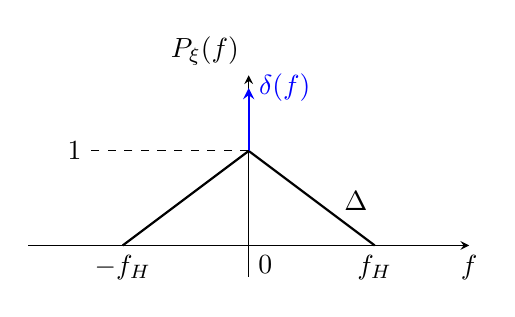
\begin{tikzpicture}[>=stealth, scale=0.8]
                % --- 坐标轴调整 ---
                \draw[->] (-3.5,0) -- (3.5,0) node[below] {$f$};
                % [修改点1]: 将纵轴标签移到左上方,避免与右侧的 delta(f) 标签打架
                \draw[->] (0,-0.5) -- (0,2.7) node[above left] {$P_{\xi}(f)$};
                % --- 三角波 ---
                \draw[thick] (-2,0) -- (0,1.5) -- (2,0);
                % [修改点2]: 将三角符号向右移动 (x坐标从 1.2 改为 1.7)
                \node at (1.7, 0.7) {$\Delta$};
                % --- 直流冲击 delta(f) ---
                % 保持粗线条和蓝色,绘制在坐标轴上方,标签在右侧
                \draw[->, thick, blue] (0,1.5) -- (0,2.5) node[right] {$\delta(f)$};
                % --- 刻度 ---
                \node[below] at (-2,0) {$-f_H$};
                \node[below] at (2,0) {$f_H$};
                \node[below right] at (0,0) {$0$};
                
                % --- 标注峰值 ---
                \draw[dashed] (0,1.5) -- (-2.5, 1.5);
                \node[left] at (-2.5, 1.5) {$1$};
            \end{tikzpicture}
        \end{center}
    
    \tcbline
    
    \textbf{1. 预备知识:傅里叶变换对的推导}
    
    为了求解本题,我们需要建立门函数 $g_{f_H}(f)$ 与抽样函数 $Sa(\cdot)$ 的对应关系。这里提供两种推导方法:
    
    \textbf{方法一:定义法 (积分推导)}
    \begin{itemize}
        \item \textbf{变量对照表}:
        \begin{center}
            \renewcommand{\arraystretch}{1.2}
            \begin{tabular}{|c|c|}
                \hline
                $\omega$ & $2\pi f$ \\
                \hline
                $f$ & $\frac{\omega}{2\pi}$ \\
                \hline
            \end{tabular}
        \end{center}
        \item \textbf{推导}:
        \[
        \begin{aligned}
            \mathcal{F}^{-1}[g_{f_H}(f)] &= \int_{-f_H/2}^{f_H/2} 1 \cdot e^{j2\pi f \tau} df \\
            &= \left[ \frac{e^{j2\pi f \tau}}{j2\pi \tau} \right]_{-f_H/2}^{f_H/2} \\
            &= \frac{e^{j\pi f_H \tau} - e^{-j\pi f_H \tau}}{j2\pi \tau} \\
            &= \frac{\sin(\pi f_H \tau)}{\pi \tau} = f_H Sa(\pi f_H \tau)
        \end{aligned}
        \]
    \end{itemize}

    \textbf{方法二:利用线性性质与尺度变换 (根据手写笔记)}
    \begin{itemize}
        \item \textbf{Step 1: 标准变换对} (门宽为 1)
        \[ g_1(f) \leftrightarrow Sa(\pi \tau) \]
        \item \textbf{Step 2: 频域尺度变换} (引入 $f_H$)
        利用性质 $X(f/k) \leftrightarrow |k|x(k\tau)$。令 $k=f_H$:
        \[ g_{f_H}(f) = g_1\left(\frac{f}{f_H}\right) \leftrightarrow f_H Sa(\pi f_H \tau) \]
        \item \textbf{Step 3: 线性性质/幅度缩放} (构造题目系数)
        题目需构造系数 $A = \frac{1}{\sqrt{f_H}}$。求 $\frac{1}{\sqrt{f_H}} g_{f_H}(f)$ 的逆变换。
        两边同乘 $\frac{1}{\sqrt{f_H}}$:
        \[ \frac{1}{\sqrt{f_H}} g_{f_H}(f) \leftrightarrow \frac{1}{\sqrt{f_H}} \cdot [f_H Sa(\pi f_H \tau)] \]
        化简右边系数 $\frac{f_H}{\sqrt{f_H}} = \sqrt{f_H}$,得最终变换对:
        \[ \boxed{\frac{1}{\sqrt{f_H}} g_{f_H}(f) \leftrightarrow \sqrt{f_H} Sa(\pi f_H \tau)} \]
    \end{itemize}

    \tcbline
    
    \textbf{2. 功率谱密度 $P_\xi(f)$ 的分解与参数求解}
    
    由图可知,$P_\xi(f) = \Delta(f) + \delta(f)$。
    
    \textbf{求解三角形 $\Delta(f)$ 的构成:}
    三角形可视为两个相同门函数 $A \cdot g_{f_H}(f)$ 的卷积。
    \[ \Delta(f) = [A \cdot g_{f_H}(f)] * [A \cdot g_{f_H}(f)] \]
    
    根据卷积几何性质:
    \begin{itemize}
        \item 卷积后高度 = $A^2 \cdot \text{门宽} = A^2 f_H$
    \end{itemize}
    
    由图知三角形顶点高度为 $1$,故 $A^2 f_H = 1 \implies A = \frac{1}{\sqrt{f_H}}$。
    即:
    \[ \Delta(f) = \left[ \frac{1}{\sqrt{f_H}} g_{f_H}(f) \right] * \left[ \frac{1}{\sqrt{f_H}} g_{f_H}(f) \right] \]

    \tcbline
    
    \textbf{3. 求解自相关函数 $R(\tau)$}
    
    利用维纳-辛钦定理及“频域卷积 $\leftrightarrow$ 时域相乘”:
    
    \[
    \begin{aligned}
        R(\tau) &= \mathcal{F}^{-1}[\Delta(f)] + \mathcal{F}^{-1}[\delta(f)] \\
        &= \mathcal{F}^{-1}\left\{ \left[ \frac{1}{\sqrt{f_H}} g_{f_H}(f) \right] * \left[ \frac{1}{\sqrt{f_H}} g_{f_H}(f) \right] \right\} + 1 \\
        &= \left( \mathcal{F}^{-1}\left[ \frac{1}{\sqrt{f_H}} g_{f_H}(f) \right] \right)^2 + 1 
    \end{aligned}
    \]
    代入步骤1中推导出的结论:
    \[
    \begin{aligned}
        R(\tau) &= \left( \sqrt{f_H} Sa(\pi f_H \tau) \right)^2 + 1 \\
        &= f_H Sa^2(\pi f_H \tau) + 1
    \end{aligned}
    \]
    
    \tcbline
    \textbf{4. 功率计算}
    \begin{itemize}
        \item 平均功率 $R(0) = f_H + 1$
        \item 直流功率 $R(\infty) = 1$
        \item 交流功率 $\sigma^2 = f_H$
    \end{itemize}
\end{examplebox}